%-----------------------------------
%-----------------------------------
\chapter{Erste Ansätze}

%------------------------------------
\section{Bestandteile eines Skeletts}

Ein Skelett besteht aus Knochen und Gelenken. Zwei Knochen sind jeweils durch ein Gelenk miteinander verbunden. Im Folgenden werden sowohl Knochen als auch Gelenke genauer beschrieben.

% Knochen
Jeder \emph{Knochen} hat sein eigenes lokales Koordinatensystem und wird zunächst als Quader dargestellt. Der Ursprung des Koordinatensystems befindet sich in einer Ecke des Quaders.
Informationen, die für die Darstellung eines Knochens erforderlich sind, sind also
seine Ausdehnung in alle drei Raumrichtungen (die Kantenlängen des Quaders) und die Position und Orientierung des Ursprungs im globalen Koordinatensystem.

% Hierarchie
Die Knochen sollten eine Hierarchie (einen Baum) bilden, da das von Algorithmen für Animationen so erwartet wird. \todo{Verweis auf previous work, wenn ausgearbeitet} Da der Wirbeltierbauplan aus Abbildung \ref{bauplan_skelett} verwendet wird, ist das auch möglich. Im Allgemeinen ist ein Skelett aber weder zusammenhängend noch ohne Kreise.

% Wurzel
Für eine Hierarchie ist ein erstes Element nötig, die Wurzel des Baums.
Dafür bietet sich ein Knochen in der Nähe des Schwerpunkts an. Oft wird hierfür die Hüfte verwendet. \todo{Beispiel/Quelle}
Da aber nicht jedes Wirbeltier eine Hüfte besitzt und es die Generierung vereinfacht, wird als Wurzelknochen ein Knochen ohne Ausdehnung in der Mitte der Rückenwirbelsäule verwendet. Dieser Knochen wird im Folgenden als \emph{Wurzelknochen} bezeichnet. Liegt Knochen $B$ in der Hierarchie direkt unter Knochen $A$, so ist $A$ der \emph{Elternknochen} von $B$ und $B$ ein \emph{Kindknochen} von $A$.

% Transformationsmatrizen
Es ist sinnvoll für jeden Knochen nicht die Position im globalen Koordinatensystem anzugeben, sondern seine Position im Koordinatensystem des Elternknochens. Verfolgt man den Pfad von einem Knochen zurück zum Wurzelknochen, so kann die Position im globalen Koordinatensystem trotzdem ausgerechnet werden. \todo{Verweis auf IK} \\
Für die Darstellung werden Transformationsmatrizen mit homogenen Koordinaten verwendet. Genauere Informationen zu diesen Transformationsmatrizen und wie sie in verschiedenen Situationen berechnet werden können sind in Absatz \ref{implementation_detail_matrices} zu finden.

% Gelenke
Ein \emph{Gelenk} ist, wie auch in der Natur, ein Verbindungsstück zwischen zwei Knochen. Es legt fest wie die beiden Knochen sich relativ zueinander bewegen können. Im Gegensatz zu echten Gelenken haben Gelenke hier aber keine Ausdehnung. Sie werden am Ende im 3D-Modell nicht dargestellt.\\
Ein Gelenk wird im Koordinatensystem des Elternknochens dargestellt. Es wird beschrieben durch seinen Abstand zum Ursprung des Elternkoordinatensystems und Bewegungseinschränkungen für den Kindknochen. Ein Gelenk kann null bis zwei Freiheitsgrade haben. Bei einem Winkel von $0^\circ$ hat das Kindelement die gleiche Ausrichtung wie das Elternelement. In Abbildung \ref{joints} sind alle Gelenke mit mindestens einem Freiheitsgrad, die im Algorithmus verwendet werden, dargestellt.

% Berechnung Transformationsmatrix des Kindelements
Ist ein Elternknochen mit einem Gelenk in einer bestimmten Ausrichtung gegeben, so lässt sich daraus die Transformationsmatrix des Kindelements berechnen.


%-----------------------------
\section{Aufbau als Grammatik}

\begin{itemize}
  \item Aufbau als Grammatik (am Ende aber für jedes Nichtterminal genau eine Regel)
  \item Aufbau der (Nicht)terminale als Baum, nur Terminale können Kinder haben, Reihenfolge der Anwendung der Regeln sollte beliebig sein
  \item Wachstum unter Berücksichtigung verschiedener Randbedingungen wie Bodenposition, Anzahl Extremitäten etc.\ Bounding Box für Nichtterminale ist dafür aber nicht nötig.
  \item Symmetrie der Skelette (spiegle Elemente zum Schluss)
  \item Repräsentation des Zustands als Hierarchie von einzelnen Komponenten (terminale sowie nichtterminale)
 \end{itemize}
 
 \begin{itemize}
  \item Iterative Erzeugung eines Skeletts durch eine probabilistische kontextfreie (?) Grammatik, die so erweitert ist, dass sie nicht ein einfaches Wort erzeugt, sondern einen Baum von Zeichen (nötig für Extremitäten). Verwendung von parametrischen L-Systemen \cite{Paramteric_L-Systems} könnte sinnvoll sein.
  
  \item Regeln sind nicht wirklich eine Grammatik, da fast jedes nichtterminale Literal nur einmal vorkommt, wenn es für jedes Körperteil andere Regeln gibt. Oder ist es möglich so zu abstrahieren, dass z.B. Arme und Beine den gleichen/ähnlichen Regeln unterliegen? Ist das sinnvoll? \todo{Abstraktionsgrad, Art der Regeln}
  Außerdem ist das Skelett nicht unbedingt zusammenhängend (siehe Biologie). $\rightarrow$ Darauf achten, dass das nicht von Algorithmus verlangt wird
  
  \item Brustbein sorgt dafür, dass Skelett nicht mehr baumartig $\rightarrow$ erstmal weglassen, ist wahrscheinlich auch nicht unglaublich relevant
  
  \item Kindelement erst erzeugen, wenn Elternelement terminal ist und Gelenk hat.
 \end{itemize}
 
 \begin{sidewaysfigure}
  \centering
  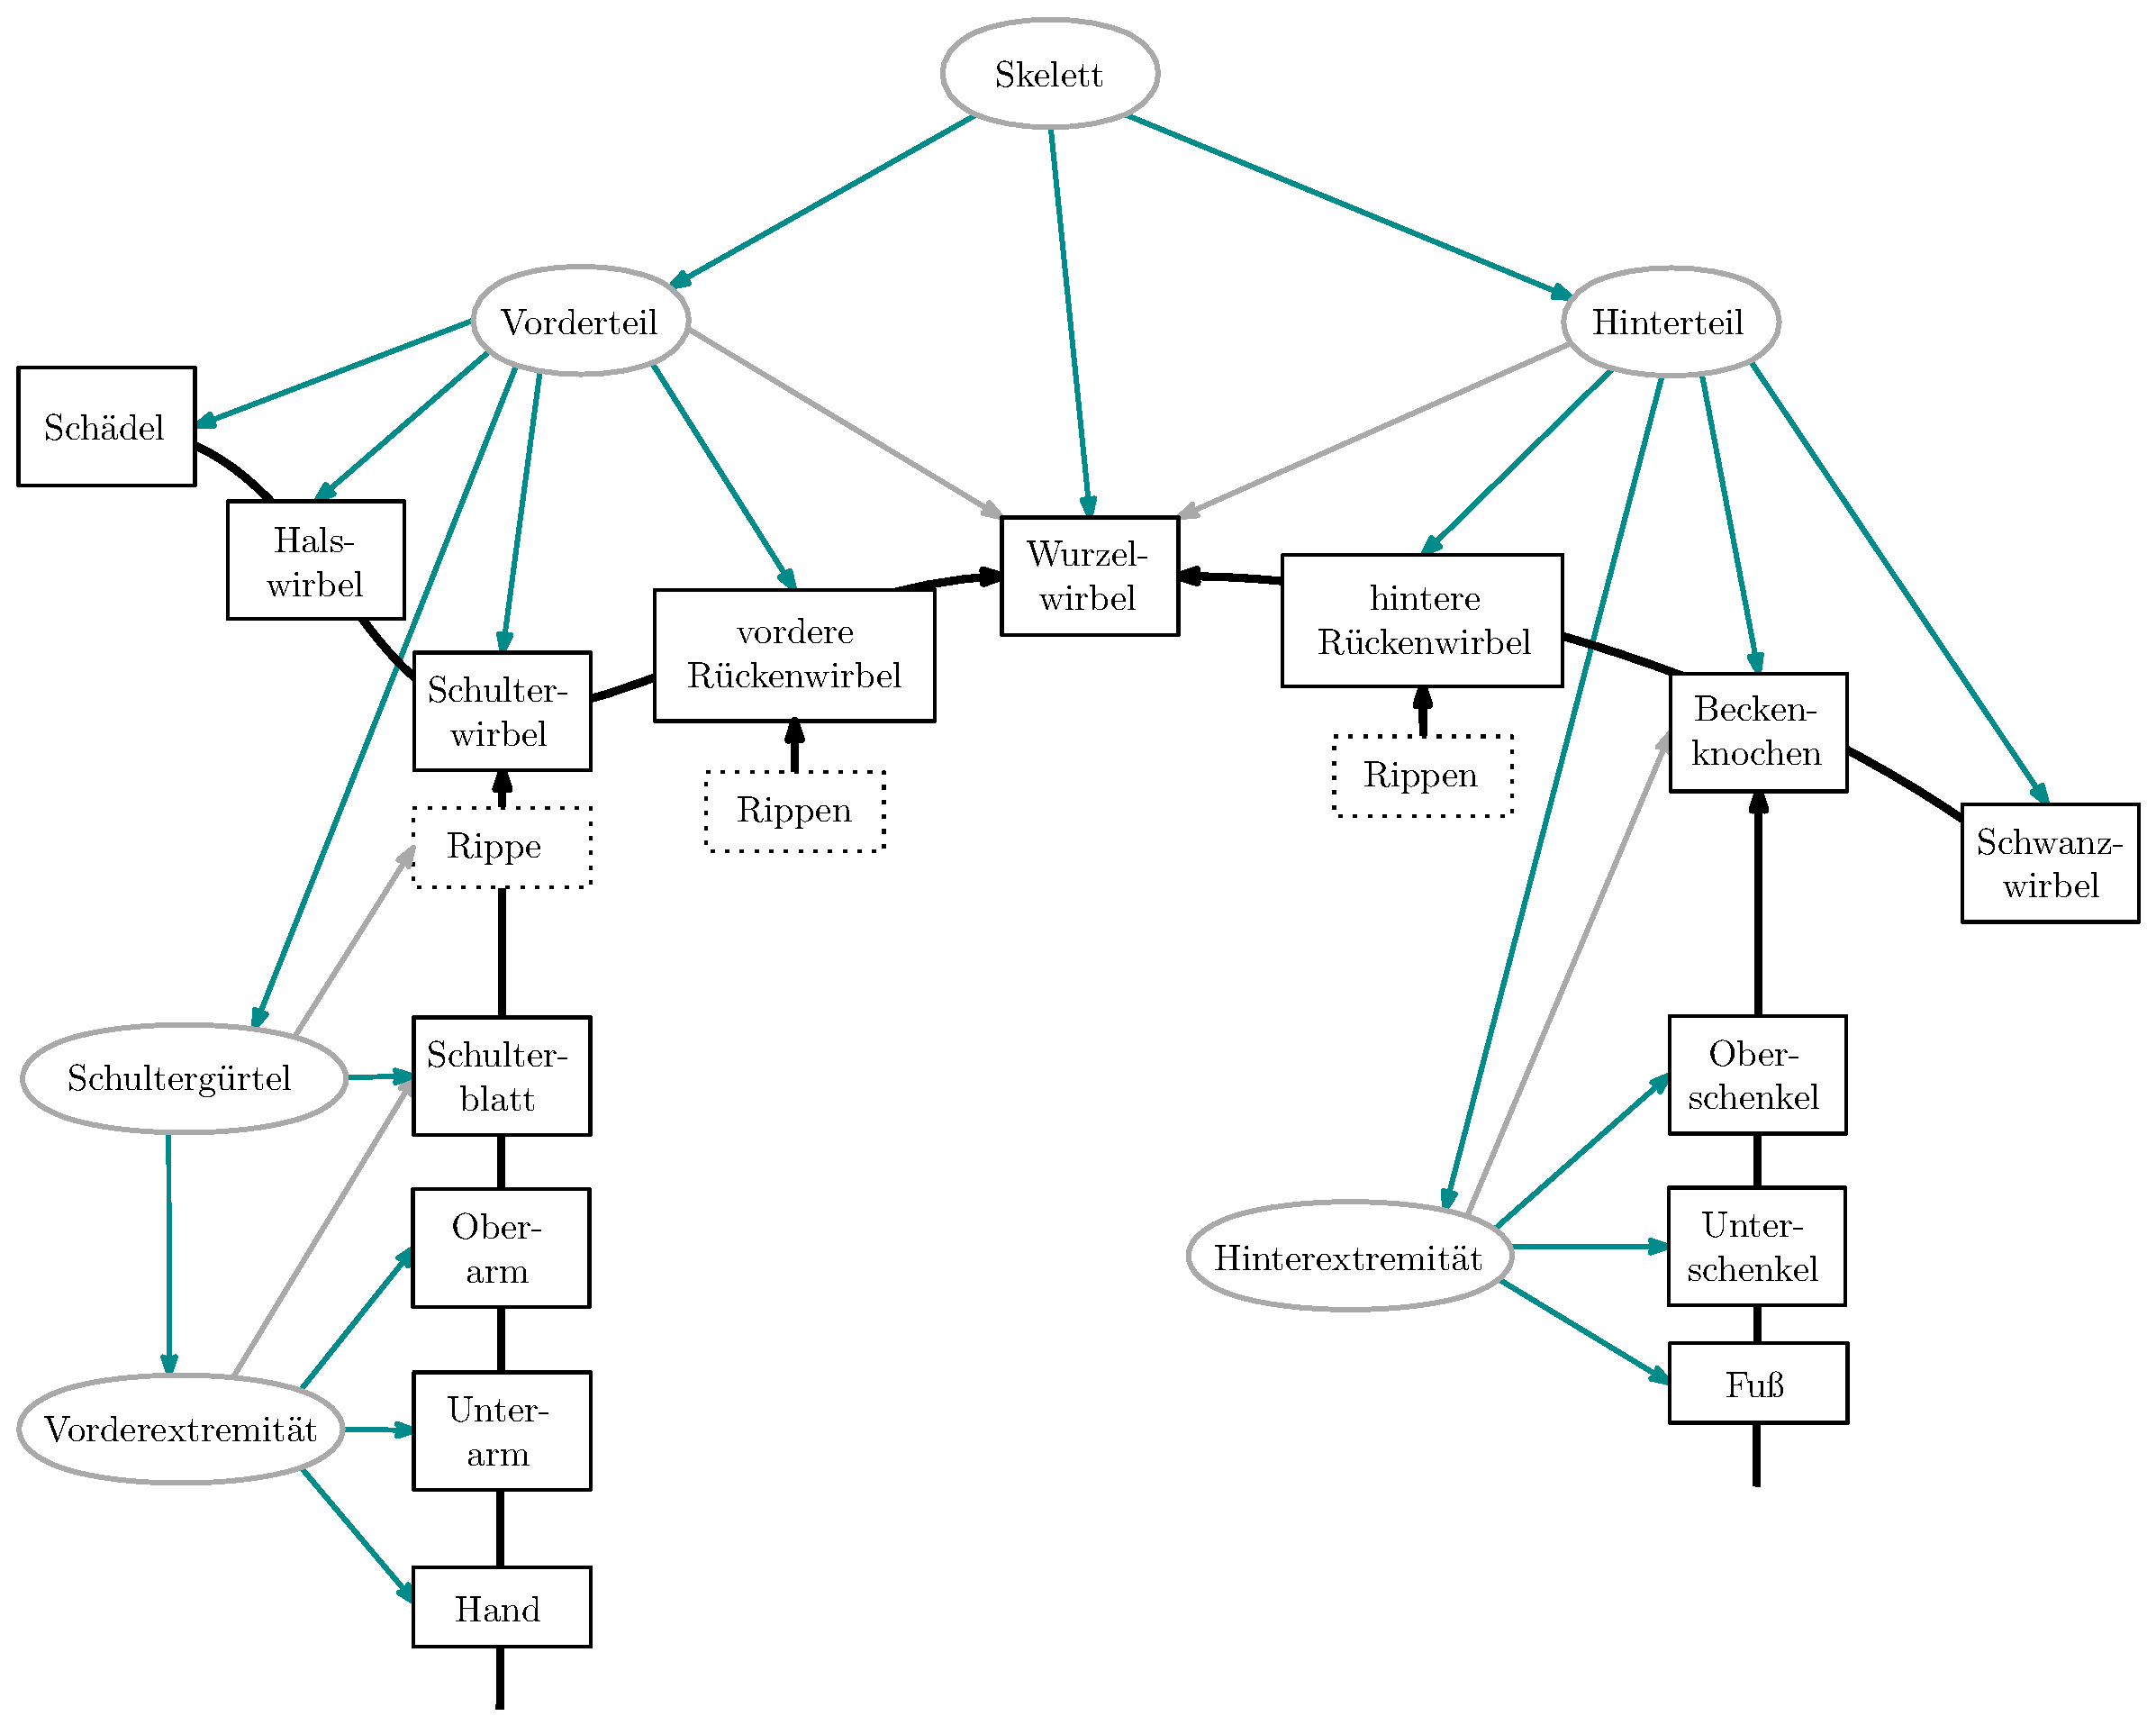
\includegraphics[height=14cm]{graphics/grammarGraph}
  \caption{Aufbau der Grammatik}
  \label{grammar_graph}
 \end{sidewaysfigure}


 

%---------------------
\section{Pose des Skeletts}

Ein Skelett ist nicht nur eine Hierarchie von Knochen, sondern wirkt auch wesentlich durch seine Pose. Das Ziel sollte also sein das Skelett in einer natürlich wirkenden Pose darzustellen, eine Pose, die das dargestellte Tier auch einnehmen würde.

% erster Ansatz: Drehmomente
Ein erster Ansatz könnte sein in jedem Schritt auszurechnen, ob das Skelett ausbalanciert ist. Dazu benötigt man den Schwerpunkt des Körpers und Position und Gewicht der Knochen.
Damit kann man dann die Drehmomente der einzelnen Knochen um den Schwerpunkt berechnen. Addieren sie sich alle zu null auf, ist das Skelett im Gleichgewicht.

% Probleme
Hierbei tauchen gleich mehrere Fragen auf:
\begin{description}
 \item[Gewicht] Wie wird das Gewicht der Knochen bestimmt? Es wird das Gewicht aller Elemente, oder zumindest das aller terminalen Elemente, benötigt. Wie wird es festgelegt? Hängt es von der Größe der Knochen ab? Außerdem müsste das ganze Gewicht des Tieres, nicht nur das der Knochen berücksichtigt werden. Wie kann bestimmt werden wieviel anderes Gewebe an einem Knochen hängt?
 
 \item[Schwerpunkt] Wo liegt der Schwerpunkt? Wird am Anfang eine große Bounding Box für das Skelett festgelegt, in deren Mitte der Schwerpunkt liegt? Verändert der Schwerpunkt seine Position je nach dem was generiert wird?
 
 \item[Gleichgewicht] Wann wird überprüft ob sich das Skelett im Gleichgewicht befindet? Ist das Gleichgewicht eine Invariante, die während der Generierung aufrecht erhalten werden soll? Oder wird es erst am Ende geprüft? Was passiert, wenn sich das Skelett nicht im Gleichgewicht befindet?
\end{description}
 
% Warum wird anderer Ansatz verwendet
Das Hauptproblem ist, dass nicht klar ist wie das Gewicht der einzelnen Körperteile bestimmt werden soll ohne zusätzlich zu den Knochen auch noch anderes Gewebe wie Muskeln oder Eingeweide zu betrachten. Deshalb wurde ein anderer Ansatz erarbeitet.
 
% Wirbelsäule als Startpunkt
Die Wirbelsäule ist ein zentraler Teil des Wirbeltierkörpers und bestimmt wesentlich das Aussehen des Skeletts.
Ihre Form variiert von relativ gerade, \zb bei Fischen oder Schlangen, bis hin zu stark geschwungenen Hälsen, \va bei Vögeln, und langen Schwänzen, \zb bei Mäusen. Außerdem zeigt sie wie aufrecht ein Tier sich hält. Große Unterschiede sind hier zwischen Fischen und auch Vierbeinern gegenüber Vögeln zu beobachten, da Vögel nur auf ihren Hinterbeinen stehen und deshalb ihr Schwerpunkt nach hinten verschoben ist. Es gibt aber auch aufrechtere Exemplare unter den "`Vierbeinern"' wie beispielsweise das Känguru oder der Tyrannosaurus Rex.\todo{Beispielbilder von Wirbelsäulen} \\
Der Mensch ist natürlich auch ein Beispiel für ein sehr aufrechtes Wirbeltier. Seine Haltung unterscheidet sich aber so stark von der der anderen Wirbeltiere, dass er hier außen vor gelassen werden soll.

Viele Knochen setzen direkt an der Wirbelsäule an, wie \zb der Kopf, die Rippen oder die Hüfte. Durch die Wirbelsäule wird also schon sehr viel vorgegeben.
Deshalb eignet sie sich sehr gut als Startpunkt für die Generierung eines Skeletts. Ausgehend von ihr kann dann der Rest des Skeletts "`wachsen"'.

% Wie Lage der Wirbelsäule bestimmen?
Wie soll aber nun die Lage der Wirbelsäule bestimmt werden?\\
Hierfür schien es sinnvoll viele Beispiele zu betrachten und Zusammenhänge zwischen verschiedenen Eigenschaften der Tiere und dem Verlauf der Wirbelsäule zu suchen.
Ein geeignetes Werkzeug hierfür ist die \emph{Principal Component Analysis} (siehe Abschnitt \ref{PCA}).

